\documentclass[letterpaper]{article}
\usepackage[submission]{aaai2027}

\usepackage[hyphens]{url}
\usepackage{graphicx}
\urlstyle{rm}
\def\UrlFont{\rm}
\usepackage{natbib}
\usepackage{caption}
\frenchspacing
\usepackage{amsmath}
\usepackage{amssymb}
\usepackage{algorithm}
\usepackage{algorithmic}
\usepackage{newfloat}
\usepackage{listings}
\usepackage{booktabs}
\usepackage{array}
\usepackage{multirow}
\usepackage{subcaption}
\usepackage{placeins}
\usepackage{enumitem}
\setcounter{topnumber}{3}
\setcounter{bottomnumber}{2}
\setcounter{totalnumber}{5}
\renewcommand{\topfraction}{0.95}
\renewcommand{\bottomfraction}{0.85}
\renewcommand{\textfraction}{0.05}
\renewcommand{\floatpagefraction}{0.85}
\DeclareCaptionStyle{ruled}{labelfont=normalfont,labelsep=colon,strut=off}
\lstset{basicstyle={\footnotesize\ttfamily},numbers=left,numberstyle=\footnotesize,xleftmargin=2em,aboveskip=0pt,belowskip=0pt,showstringspaces=false,tabsize=2,breaklines=true}
\floatstyle{ruled}
\newfloat{listing}{tb}{lst}{}
\floatname{listing}{Listing}
\pdfinfo{
/TemplateVersion (2027.1)
}

\newcommand{\hist}{h}
\newcommand{\action}{a}
\newcommand{\obs}{o}
\newcommand{\effect}{e}
\newcommand{\progress}{\Delta^{\mathrm{prog}}}
\newcommand{\basepol}{\pi_0}
\newcommand{\controller}{\pi_{\mathrm{ACE}}}
\newcommand{\aceop}{\omega}
\newcommand{\Pass}{\mathrm{Pass@1}}
\newcommand{\Raw}{\mathrm{Raw}}
\newcommand{\Rule}{\mathrm{Rule}}
\newcommand{\Learned}{\mathrm{Adapter{+}Learned}}
\newcommand{\FunctionalLoop}{\operatorname{Functional\ Loop}}


\setcounter{secnumdepth}{0}
\title{Escaping Degenerate Functional Loops:\\ Learning Programmatic Action Recovery for Tool-Using LLMs}
\author{Anonymous Submission}
\affiliations{}

\begin{document}
\maketitle

\begin{abstract}
Tool-using large language models (LLMs) extend text generation to multi-step interaction with APIs, databases, and external services, where reliable execution requires every tool call to translate into task progress. In this paper, we find that this requirement is frequently violated: after a task is blocked, a tool-using LLM may keep issuing different tool calls whose observations repeat the same unresolved effect on the visible task state. We refer to such episodes as \emph{Functional Loops}, and our analysis on three benchmarks and four LLMs shows that they are prevalent, coincide with lower task performance, and are not well captured by string-level tool repetition. To escape a Functional Loop through a grounded local correction, we propose \textbf{LoopBreaker}, a local recovery layer that reuses concrete training-time failures at inference time. During training, LoopBreaker compiles recurring failure patterns into typed Recovery Cards, each pairing a state-sensitive trigger with a grounded and bounded action program. At inference time, a frozen controller admits at most one eligible Card once a Functional Loop is detected, and then returns control to the base LLM. Experiments across three tool-use benchmarks and nine LLMs show that LoopBreaker consistently improves the primary task outcome, and reduces tool calls on Functional Loop-exposed trajectories\footnote{Code and data are available in supplementary materials.}.
\end{abstract}

\section{Introduction}

Tool-using large language models (LLMs)~\citep{yao2023react,schick2023toolformer,qin2023toollm} extend LLMs from text generation to multi-step interaction with APIs, databases, and external services, showing strong performance on a growing range of real-world tool-use tasks~\citep{yao2024taubench,barres2025tau2bench,trivedi2024appworld,lu2025toolsandbox,chen2025acebench,he2026vitabench}. Reliable execution demands more than selecting a syntactically valid call, since each interaction step should translate into progress on the underlying task.

However, we find that a tool-using LLM often expends interaction budget without producing progress. After a task is blocked, the LLM may keep issuing different tool calls whose observations repeat the same unresolved effect on the visible task state, and every additional call consumes a step without moving the task closer to completion. For instance, in a STATE-Bench Shopping task with a hard \$100 budget, the LLM can spend six tool calls searching, retrieving details of an over-budget item, and querying promotions, and none of them repairs the budget violation. We refer to such an episode as a \emph{Functional Loop}, and our analysis across three benchmarks and four LLMs indicates that it is prevalent, is associated with lower task performance, and is not well captured by string-level tool repetition (Section~\ref{sec:functional-loops}).

\begin{figure}[t]
    \centering
    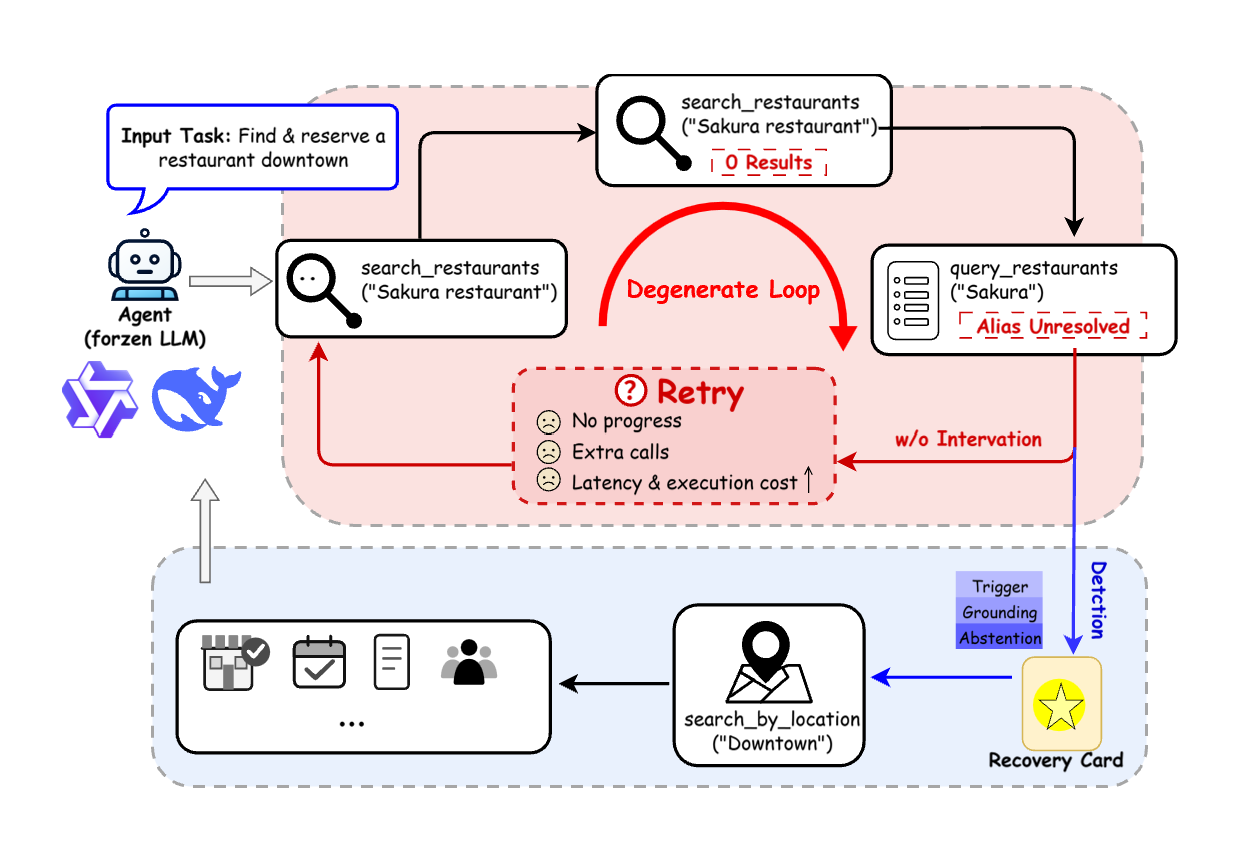
\includegraphics[width=\columnwidth]{figures/fig_persist_ace_escape_overview.png}
    \caption{An illustrative functional loop and a local escape by LoopBreaker. Different tool calls repeat the same unresolved effect after feedback is visible, and LoopBreaker admits a grounded location-search Card, applies one bounded correction, and returns control to the base LLM.}
    \label{fig:escape-example}
\end{figure}

Prior work approaches related failure modes from three directions. Early-exit methods reduce ineffective behavior by deciding when to halt a running trajectory~\citep{lu2025runaway}, while termination alone does not repair a state that a small correction could still resolve. Test-time replanning proposes a recovery plan through another generation step~\citep{kim2026rein,shinn2023reflexion}, while the recovery action is only as reliable as the underlying model and adds an unbounded generation cost. Policy optimization treats execution errors as training signals and updates the model with reinforcement learning~\citep{zhang2026fission,kang2026trace,zhang2026pivot,ta2026reinforced}, and requires gradient access that is unavailable for many production LLMs. Overall, these approaches either halt too early, act without a grounded correction, or rely on write access to model parameters, and none of them treats a Functional Loop as a distinct recoverable execution state.

In this paper, we aim to escape a Functional Loop through a grounded local correction, while leaving the base LLM's policy unchanged. To this end, we begin by asking a foundational question: \emph{when a Functional Loop is detected, what form of correction can be admitted conservatively?} A useful correction should be tied to a specific failure signature, executable in the environment, and admissible only when its trigger and grounding conditions are satisfied. Along with this idea, we propose \textbf{LoopBreaker}, a local recovery layer that reuses concrete training-time failures at inference time. As shown in Figure~\ref{fig:framework}, LoopBreaker mines recurring failure patterns in training trajectories offline and compiles each pattern into a typed Recovery Card that pairs a state-sensitive trigger with a grounded and bounded action program. At inference time, a frozen controller admits at most one eligible Card once a Functional Loop is detected, and immediately returns control to the base LLM.

In summary, our key contributions are three-fold.
\begin{itemize}[leftmargin=1em, itemsep=-1ex, topsep=0.2ex]
    \item \textbf{Functional Loop Analysis:} To the best of our knowledge, this is the first systematic study of Functional Loops in tool-using LLMs. We formalize a Functional Loop as a feedback-visible sequence that makes no task progress and repeats the same unresolved effect, and characterize its prevalence and impact across four LLMs and three benchmarks.
    \item \textbf{LoopBreaker:} We propose LoopBreaker, which pairs an offline experience compiler with an online selective controller, and turns concrete training failures into grounded and bounded recovery programs at inference time.
    \item \textbf{Strong Performance:} Experiments across three tool-use benchmarks~\citep{lu2025toolsandbox,zhang2026deepplanning,shi2026tauknowledge} and nine LLMs show that LoopBreaker consistently improves the primary task outcome, with particularly strong gains on Functional Loop-exposed trajectories.
\end{itemize}


\section{Functional Loops in Tool-Using LLMs}
\label{sec:functional-loops}

Functional Loops describe a class of tool-use episodes that consume interaction budget without moving the task forward. We formalize the concept below, and then show three properties that make it a well-defined target for recovery: it is prevalent across models and environments, it degrades task performance, and it is not captured by string-level tool repetition.

\noindent\textbf{Definition.}\quad
For a tool-use trajectory $\tau=(s_0,a_0,o_0,\ldots,s_T)$, we summarize the visible task state at step $t$ as $q_t=(E_t,S_t,U_t)$, with $E_t$ the non-redundant evidence, $S_t$ the task-relevant environment state, and $U_t$ the set of unresolved requirements. The functional effect of $a_t$ is $e_t=(\Delta E_t,\Delta S_t,\Delta U_t,f_t)$, with $f_t$ a failure signature and $\kappa(e_t)$ a canonicalization for comparison.

Let $p_t=1$ when $a_t$ either adds new evidence, moves state toward an unresolved requirement, or produces a new failure signature. To make the definition applicable at inference time, we evaluate progress and repetition over the trailing history $H_t=\{t-w,\ldots,t-1\}$:
\begin{equation}
\begin{aligned}
N(t)&=\mathbb{I}\!\left[U_t\neq\varnothing\ \land\ \sum_{j\in H_t}p_j=0\right],\\
R_e(t)&=\mathbb{I}\!\left[
\substack{\exists i<j,\ i,j\in H_t:\\
\kappa(e_i)=\kappa(e_j)\ \land\ o_i\prec a_j}\right],
\end{aligned}
\end{equation}
where $o_i\prec a_j$ means $o_i$ was visible before $a_j$ was proposed. A Functional Loop at step $t$ is then
\begin{equation}
\mathcal{L}(t)=N(t)\land R_e(t),
\label{eq:functional-loop}
\end{equation}
and a trajectory is \emph{Functional Loop-exposed} if it contains such an episode. Tool identity is irrelevant: a Functional Loop is defined at the level of functional effects.

\noindent\textbf{Functional Loops are Prevalent Across Models and Environments.}\quad
We first ask how common such loops are among failed trajectories, and whether their prevalence depends on the base model or on the surrounding environment. Figure~\ref{fig:functional-loop-prevalence} separates the two sources of variation. Under the same failed STATE-Bench tasks, Qwen3-14B enters a functional loop in $35.2\%$ of its failed trajectories, whereas DeepSeek-v4-Flash, MiMo-v2.5-Pro, and DeepSeek-v4-Pro loop far less often. With DeepSeek-v4-Flash held fixed, prevalence rises to $76.0\%$ on DeepPlanning Shopping and $52.8\%$ on $\tau$-Knowledge, well above the $5.1\%$ observed on STATE-Bench. Functional loops therefore reflect an interaction between the model's tool policy and the environment, and are especially frequent on long-horizon planning tasks.

\begin{figure}[t]
  \centering
  \begin{subfigure}[b]{0.48\columnwidth}
    \centering
    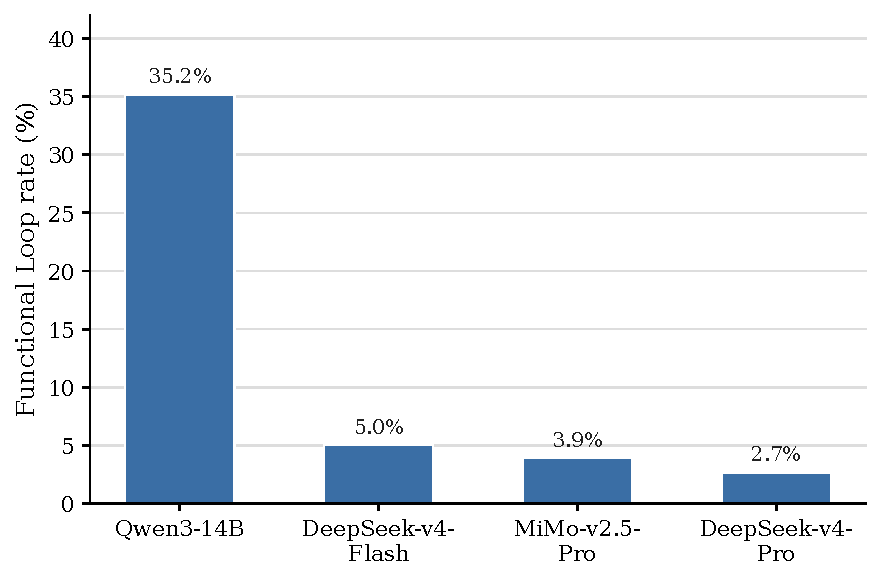
\includegraphics[width=\linewidth]{figures/fig_prevalence_by_model.pdf}
    \caption{Varying model on STATE-Bench.}
    \label{fig:prev-by-model}
  \end{subfigure}
  \hfill
  \begin{subfigure}[b]{0.48\columnwidth}
    \centering
    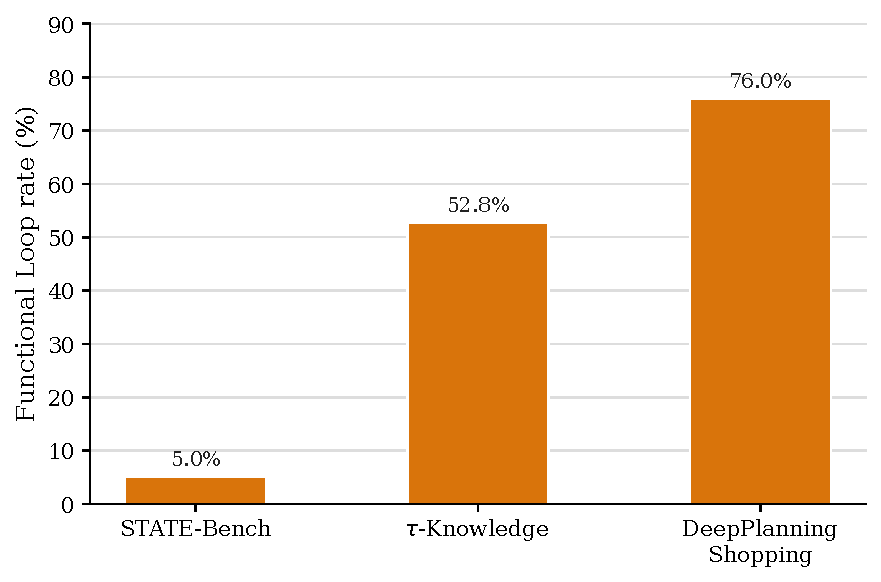
\includegraphics[width=\linewidth]{figures/fig_prevalence_by_benchmark.pdf}
    \caption{Varying benchmark under DS-v4-Flash.}
    \label{fig:prev-by-benchmark}
  \end{subfigure}
  \caption{Functional Loops are prevalent among failed trajectories. (a) With STATE-Bench held fixed, the Functional Loop rate varies from $2.7\%$ to $35.2\%$ across four tool-using LLMs. (b) With DeepSeek-v4-Flash held fixed, the rate rises to $76.0\%$ on DeepPlanning Shopping and $52.8\%$ on $\tau$-Knowledge, far above STATE-Bench.}
  \label{fig:functional-loop-prevalence}
\end{figure}

\noindent\textbf{Functional Loops Coincide with Lower Task Performance.}\quad
We next test whether the presence of a functional loop is associated with degraded task performance. Figure~\ref{fig:statebench-fl-consequence} compares STATE-Bench trajectories with and without a functional loop. Exposed trajectories score lower for every evaluated model and use $1.6$--$2.6\times$ more tool calls per trajectory. The pattern is observational, and difficult tasks may both invite longer interaction and fail more often. Even so, the association identifies a costly execution state that consumes interaction budget without changing the state that blocks completion.

\begin{figure}[t]
  \centering
  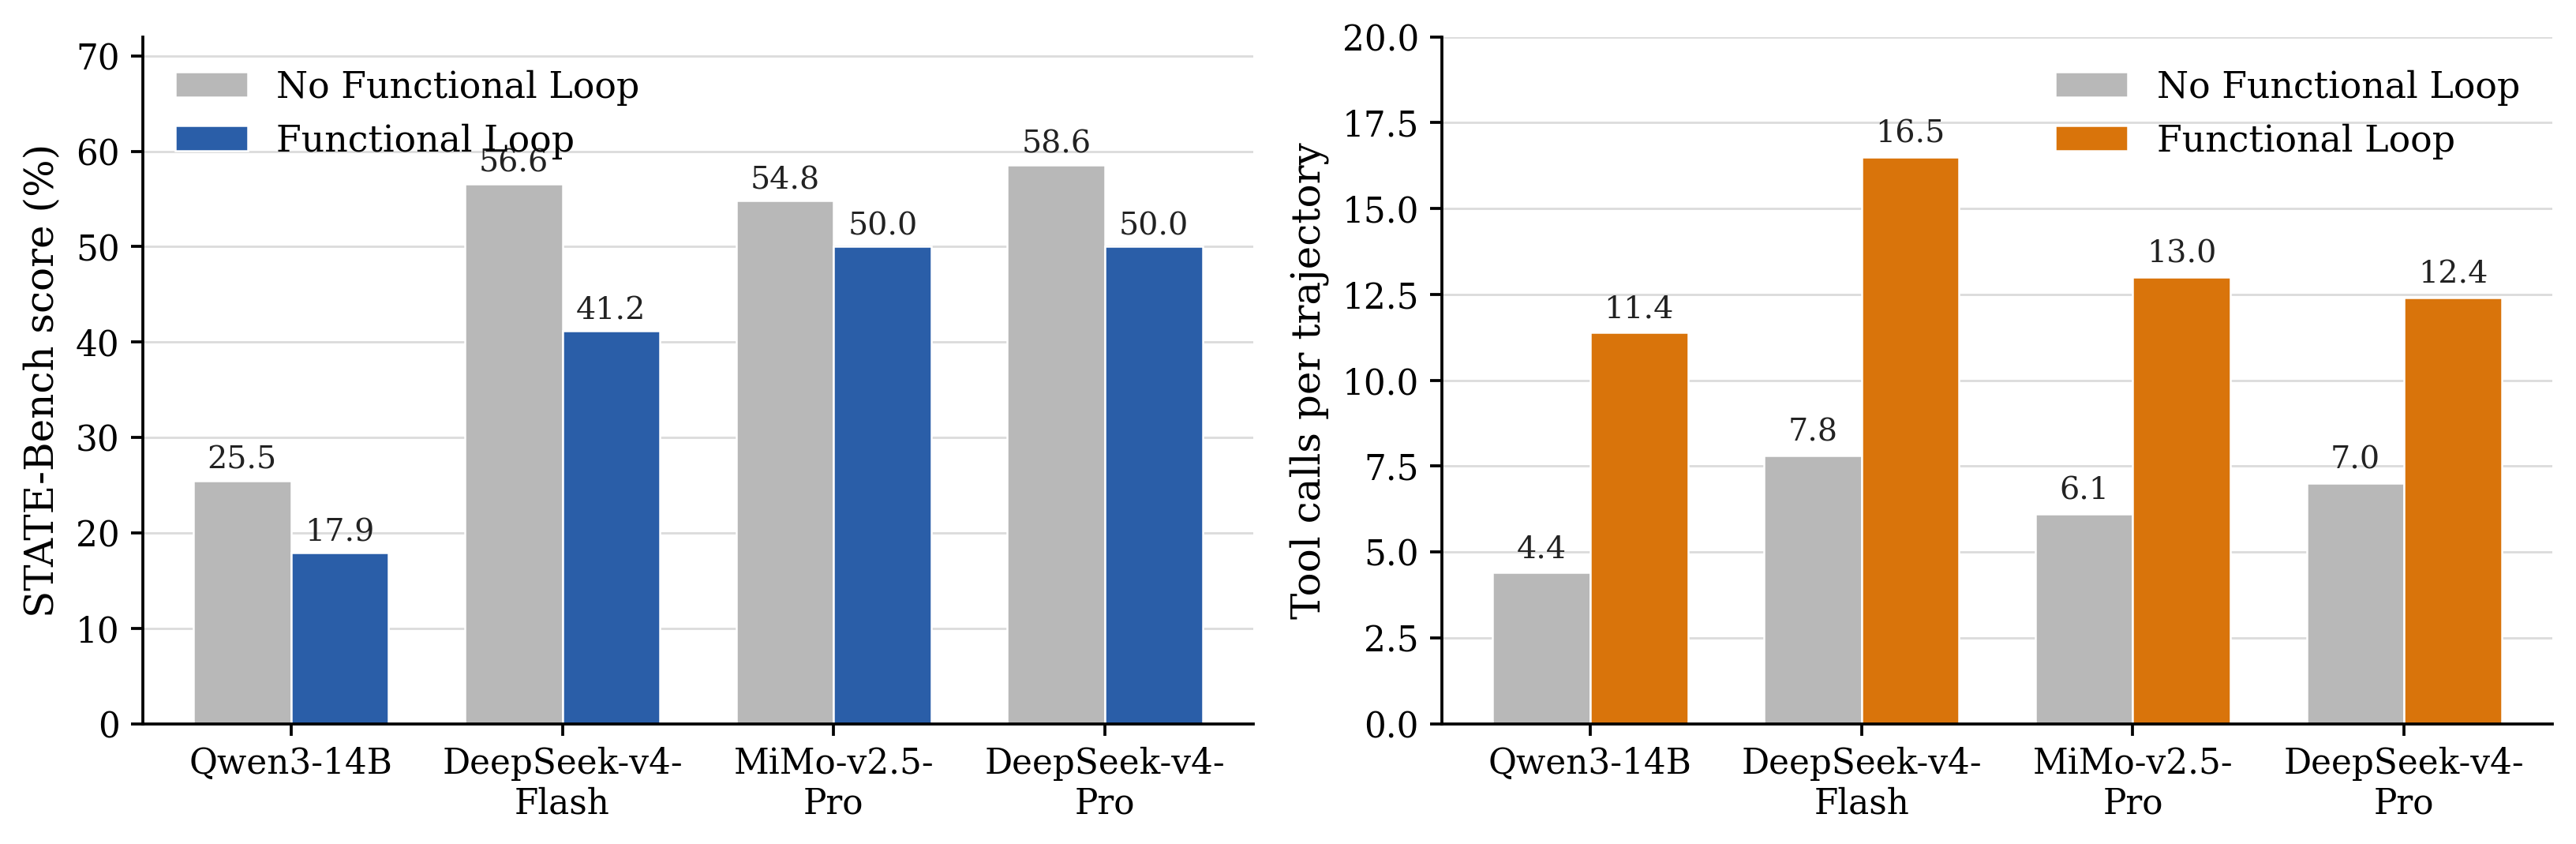
\includegraphics[width=\columnwidth]{figures/fig_fl_statebench_consequences.png}
  \caption{Functional Loop-exposed STATE-Bench trajectories obtain lower scores and consume $1.6$--$2.6\times$ more tool calls than unexposed ones for every evaluated model.}
  \label{fig:statebench-fl-consequence}
\end{figure}

Table~\ref{tab:cross-tool-fl-case} traces a representative baseline STATE-Bench Shopping trajectory in which DeepSeek-v4-Flash searches for wireless headphones under a hard \$100 budget. The first two searches produce a new failure signature, and the third search reveals a \$110 item; neither counts as no-progress under our definition. The functional loop begins from Step 4, after the over-budget candidate is confirmed: subsequent queries against the account and promotions repeat the same unresolved budget effect. A functional loop is therefore a signal to consider recovery, and does not by itself imply that the trajectory should be terminated.

\begin{table}[t]
\centering
\scriptsize
\setlength{\tabcolsep}{2pt}
\begin{tabular}{@{}>{\raggedright\arraybackslash}p{0.06\columnwidth}>{\raggedright\arraybackslash}p{0.32\columnwidth}>{\raggedright\arraybackslash}p{0.28\columnwidth}>{\raggedright\arraybackslash}p{0.24\columnwidth}@{}}
\toprule
Step & Tool Action & Feedback & Functional Effect \\
\midrule
1--2 & \texttt{search\_products}\newline ($\leq\$100$) & No matching headphones & No feasible item \\
3 & \texttt{search\_products}\newline ($\leq\$1000$) & Finds a \$110 candidate & Budget violated \\
4 & \texttt{get\_product\_details} & Confirms the \$110 price & Violation persists \\
5--6 & Account and promotion queries & No benefit or discount & Constraint unresolved \\
\bottomrule
\end{tabular}
\caption{A cross-tool Functional Loop from STATE-Bench Shopping. Steps 4--6 form the Functional Loop: different tools preserve the same unresolved budget violation once the over-budget candidate has been confirmed.}
\label{tab:cross-tool-fl-case}
\end{table}

\noindent\textbf{Tool-Name Repetition is a Weak Proxy.}\quad
An obvious alternative is to identify a stalled state by inspecting consecutive tool names. Figure~\ref{fig:same-tool-repeat} groups STATE-Bench trajectories by whether the same tool is called consecutively. Score differences between the two groups are small and even change direction across models, indicating that string-level repetition is a weak signal for the underlying execution problem. Two different tools can produce the same functional effect on the visible task state, and a second call to the same tool can still produce new evidence. Reasoning at the level of functional effects therefore provides a more useful boundary for recovery.

\begin{figure}[t]
  \centering
  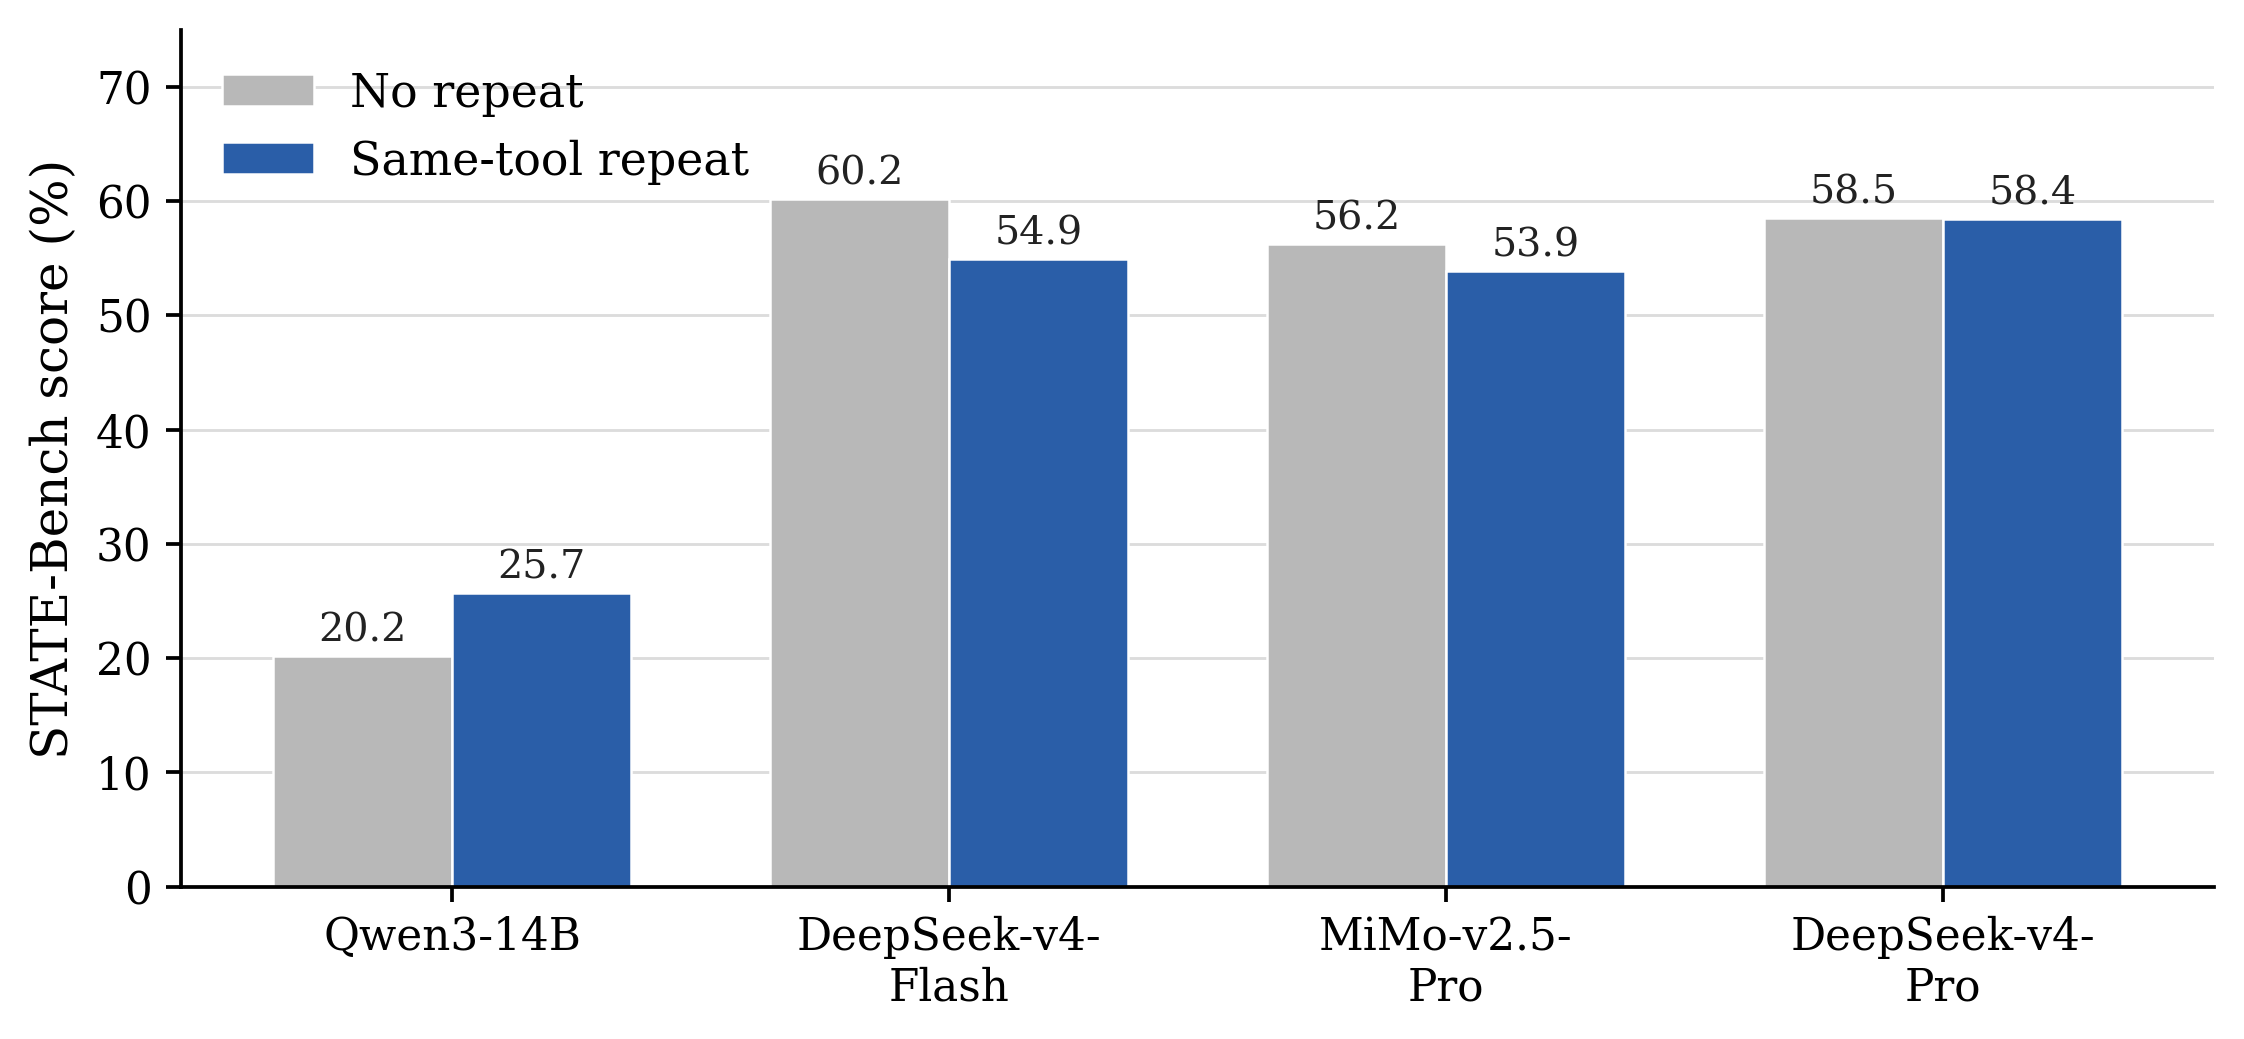
\includegraphics[width=\columnwidth]{figures/fig_statebench_same_tool_repeat.png}
  \caption{Consecutive same-tool calls are a weak proxy for unresolved effect: STATE-Bench scores are close between the two groups, and the sign of the difference varies across models.}
  \label{fig:same-tool-repeat}
\end{figure}

\begin{figure*}[t]
\centering
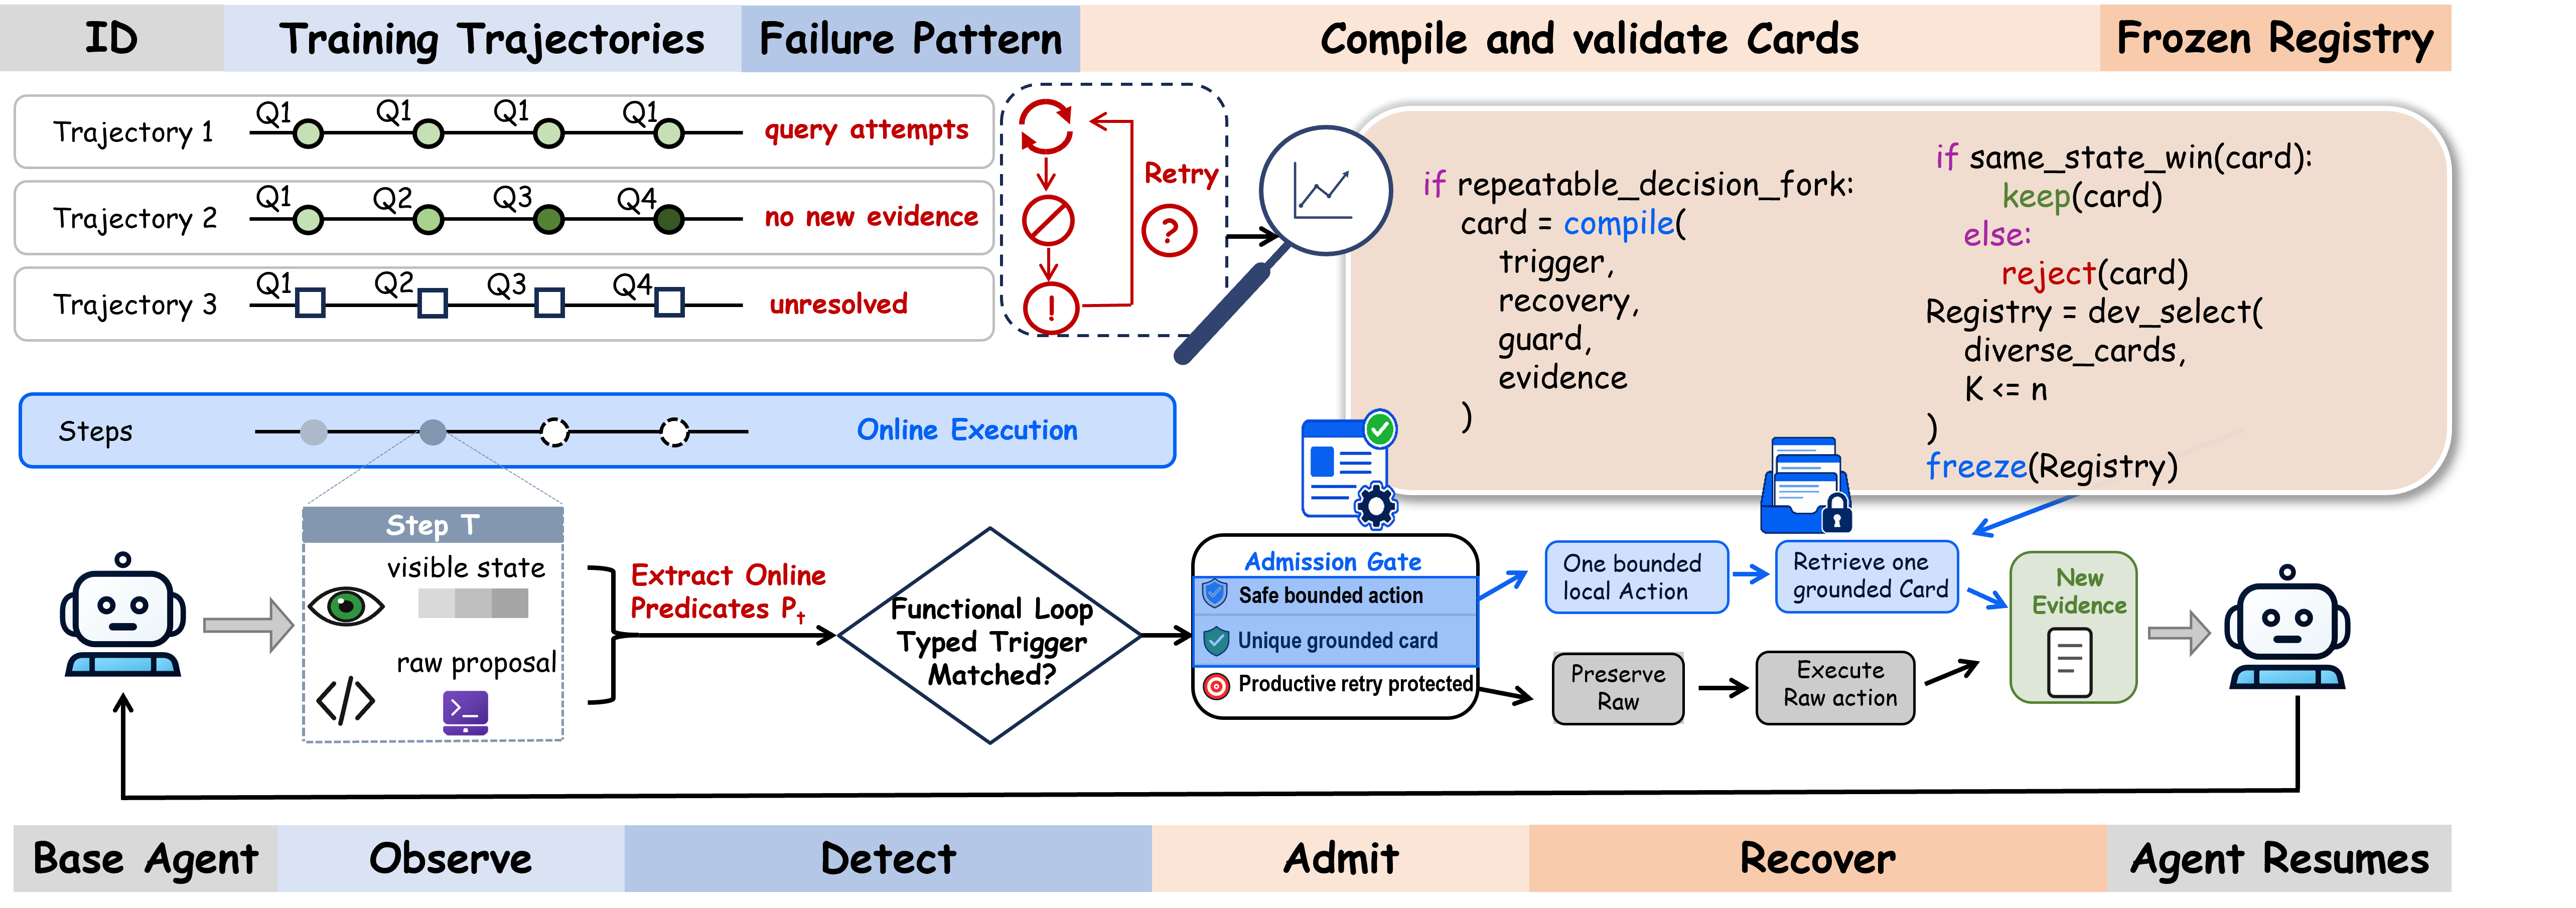
\includegraphics[width=0.98\textwidth]{figures/fig_persist_ace_pipeline.png}
\caption{Overview of LoopBreaker. The offline path mines recurring failure patterns in training trajectories, compiles each pattern into a typed Recovery Card, and stores validated Cards in a frozen benchmark-specific Registry. The online path detects a Functional Loop, admits at most one eligible Card, executes the resulting action in the environment, and returns control to the base LLM.}
\label{fig:framework}
\end{figure*}


\section{LoopBreaker}
\label{sec:method}

LoopBreaker is a local recovery layer for tool-using LLMs. Its central idea is to \emph{reuse concrete training-time failures} as inference-time experience: once a Functional Loop is detected, a validated local program repairs it without a fresh generation step, so the base LLM is left unchanged. As shown in Figure~\ref{fig:framework}, LoopBreaker realizes this idea in two stages. During training, recurring failure patterns are compiled from trajectories into typed Recovery Cards. At inference time, a frozen controller admits at most one eligible Card at a matched Functional Loop. Each Card is a typed local program with an executable body, grounded arguments, and a bounded budget, and admission is deterministic. When the trigger, grounding, or validity check fails, LoopBreaker preserves the baseline action.

\subsection*{Offline Compilation}

\textbf{Mine Failure Patterns.}\quad
The upper path of Figure~\ref{fig:framework} starts from one benchmark's training trajectories. Failed prefixes form a noisier signal than successful trajectories, since most of them do not admit a unique repair. LoopBreaker therefore admits only prefixes that satisfy Eq.~\ref{eq:functional-loop}, and among these it retains a candidate only if the failure pairs with an executable and grounded replacement. Concretely, at each pre-action prefix, $N$ recalls a no-progress state and $\kappa(e)$ tests whether feedback-visible calls repeat the same unresolved effect. We represent a candidate as
\begin{equation}
x_i=\left(s_i,a_i,e_i,\Delta E_i,\Delta S_i,u_i,\hat a_i,g_i,r_i\right),
\label{eq:candidate}
\end{equation}
where $\hat a_i$ is an executable replacement, $g_i$ is its visible grounding source, and $r_i$ is a risk tag. A replacement may repair an argument or a blocked prerequisite, and cannot invent entities or relax user constraints. Candidates are then grouped by unresolved effect, action transition, and grounding source.

\textbf{Compile and Validate Cards.}\quad
Each supported group is compiled into a typed Recovery Card
\begin{equation}
c=(z_c,\phi_c,\psi_c,\rho_c,g_c,b_c,r_c),
\label{eq:card}
\end{equation}
where $z_c$ identifies the failure family, $\phi_c$ the trigger, $\psi_c$ the abstention guards, $\rho_c$ the executable program, $g_c$ the grounding rule, $b_c$ the budget, and $r_c$ the risk tag. A Card is therefore a typed local program with executable arguments, and its trigger and effect are both verifiable in the environment. When snapshots are available, baseline and Card actions are compared from the same state; otherwise we use paired execution without claiming same-state evidence. Retention is gated by task outcome and execution validity, while loop and cost measures serve as diagnostics.

\textbf{Freeze the Registry.}\quad
We reject candidates that rely on future or test-time information, ambiguous entities, or constraint violations. Every Card definition together with the controller's runtime settings is frozen before held-out testing. Training-time induction is protocol-constrained: a coding LLM may normalize training failures and instantiate the fixed Card schema, and researchers set the retention protocol without accessing test tasks or outcomes.

\subsection*{Online Recovery}

\textbf{Observe and Detect.}\quad
In the lower path of Figure~\ref{fig:framework}, the LLM receives tool feedback and proposes a baseline action $a_t$. Observe exposes the visible history and state $s_t$, and Detect applies Eq.~\ref{eq:functional-loop}: $N=1$ recalls no progress, and $R_e=1$ confirms a repeated feedback-visible effect. Detection therefore reasons at the level of \emph{functional effects}, so a surface tool-name repeat alone is not sufficient to trigger recovery. Detection alone does not authorize intervention.

\textbf{Admit.}\quad
The controller then retrieves Cards whose trigger matches the current functional loop family. The eligible set at step $t$ is
\begin{equation}
\begin{aligned}
\mathcal{C}_t=\{c\in\mathcal{R}:{}&\phi_c(s_t,a_t)=1\land\psi_c(s_t,a_t)=0\land b_c>0,\\
&\operatorname{Unique}(g_c(s_t))=1\land\operatorname{Valid}(\rho_c(s_t,a_t))=1\},
\end{aligned}
\label{eq:eligible}
\end{equation}
where $\phi_c$ matches the state and effect, $\psi_c$ protects productive retries, and $b_c$ is the remaining budget. Admission also requires unique grounding and a schema-valid, constraint-preserving action. A frozen priority order favors smaller changes and stronger grounding. When recent progress, ambiguous grounding, or a failed validity check is present, LoopBreaker preserves the baseline proposal. This selective admission is what keeps a mined Card from harming a productive retry, and its practical value is quantified in Section~\ref{sec:analysis}.

\textbf{Recover and Resume.}\quad
For the highest-priority admitted Card $c^\star$, the executed policy is
\begin{equation}
\pi_{\mathrm{LB}}(s_t,a_t)=
\begin{cases}
\rho_{c^\star}(s_t,a_t), & \mathcal{C}_t\neq\varnothing,\\
a_t, & \mathcal{C}_t=\varnothing.
\end{cases}
\label{eq:controller}
\end{equation}
The environment executes the admitted Card program or the baseline action, and control returns to the LLM. Cards cannot invoke one another without an intervening LLM proposal, so LoopBreaker keeps the base LLM in charge of the trajectory.


\section{Experiments}
\label{sec:experiments}

We compare baseline tool-using LLMs against the same models equipped with LoopBreaker. Official task measures are primary, and functional-loop behavior and tool cost are reported as execution diagnostics.

\subsection*{Benchmarks}

\textbf{STATE-Bench}~is a stateful conversational tool-use benchmark. STATE-Bench v0.8.1 contains $50$ held-out tasks in each of Travel, Customer Support, and Shopping Assistant. Following the official protocol, Pass@1 is the average completion rate over five runs per task, Pass$^5$ is the fraction of tasks completed in all five runs, and UX averages the user-experience score on valid judged trajectories.

\textbf{DeepPlanning}~\citep{zhang2026deepplanning} is a benchmark for long-horizon agentic planning under verifiable constraints. We use its $120$-task Shopping Planning split, and report Match Score and Case Accuracy.

\textbf{$\tau$-Knowledge}~\citep{shi2026tauknowledge} evaluates knowledge-intensive tool use over $97$ tasks, in which the LLM must retrieve and reason over unstructured documents. We report Reward mean, Pass$^1$--Pass$^4$, Action Recall, and Document Recall.

\subsection*{Experimental Setup}

We keep Card construction strictly separate from held-out evaluation. Training trajectories are used to mine failure patterns and instantiate Cards, and a development split is used to select the Registry. Every Card definition together with the controller's runtime settings is frozen before test execution.

We evaluate nine LLMs on STATE-Bench (five runs per task), six LLMs on DeepPlanning Shopping (four runs per task), and five model-version pairs on $\tau$-Knowledge (four runs per task). For each LLM, Baseline uses the base model and LoopBreaker adds the same frozen benchmark-specific Registry, while tasks, tools, simulator, and evaluator are otherwise unchanged. Compilation is run independently per benchmark, so Cards are never pooled across environments.

\begin{table}[!t]
\centering
\small
\setlength{\tabcolsep}{3pt}
\renewcommand{\arraystretch}{1.05}
\resizebox{\columnwidth}{!}{%
\begin{tabular}{llccc}
\toprule
Setting & Model & Pass@1 (\%) & Pass$^5$ (\%) & UX \\
\midrule
\multirow{9}{*}{Baseline} & Ministral-3-14B & 30.50 & 8.70 & 2.95 \\
 & Qwen3-14B & 24.00 & 7.30 & 2.90 \\
 & GPT-5.5 & 56.67 & 34.00 & 3.76 \\
 & Claude-Sonnet-5 & 62.00 & 36.67 & 4.07 \\
 & Claude-Opus-4-8 & 57.47 & 30.00 & 4.02 \\
 & DeepSeek-v4-Flash & 56.90 & 30.00 & 3.72 \\
 & DeepSeek-v4-Pro & 59.10 & 34.00 & 3.93 \\
 & MiMo-v2.5-Pro & 54.50 & 27.30 & 3.96 \\
 & GPT-5.6-Sol & 62.13 & 39.33 & 3.93 \\
\midrule
\multirow{9}{*}{LoopBreaker} & Ministral-3-14B & 30.90 (\textbf{+0.40}) & 11.30 (\textbf{+2.60}) & 2.96 (+0.01) \\
 & Qwen3-14B & 26.80 (\textbf{+2.80}) & 10.00 (\textbf{+2.70}) & 2.90 (0) \\
 & GPT-5.5 & 60.80 (\textbf{+4.13}) & 35.33 (\textbf{+1.33}) & 3.79 (+0.03) \\
 & Claude-Sonnet-5 & 62.80 (\textbf{+0.80}) & 36.00 ($-0.67$) & 4.05 ($-0.02$) \\
 & Claude-Opus-4-8 & 59.33 (\textbf{+1.86}) & 30.67 (\textbf{+0.67}) & 4.05 (+0.03) \\
 & DeepSeek-v4-Flash & 59.50 (\textbf{+2.60}) & 34.00 (\textbf{+4.00}) & 3.75 (+0.03) \\
 & DeepSeek-v4-Pro & 59.50 (\textbf{+0.40}) & 34.00 (0) & 3.94 (+0.01) \\
 & MiMo-v2.5-Pro & 56.30 (\textbf{+1.80}) & 27.30 (0) & 3.96 (0) \\
 & GPT-5.6-Sol & 62.67 (\textbf{+0.54}) & 38.67 ($-0.66$) & 3.96 (+0.03) \\
\bottomrule
\end{tabular}%
}
\renewcommand{\arraystretch}{1.0}
\caption{Overall STATE-Bench test results. Each setting contains $150$ tasks and five trials, with a fixed $750$-trajectory Pass@1 denominator. Values in parentheses report LoopBreaker minus Baseline; positive gains are in \textbf{bold}. UX averages valid judged trajectories.}
\label{tab:state-main}
\end{table}

\begin{table}[!t]
\centering
\small
\setlength{\tabcolsep}{3pt}
\renewcommand{\arraystretch}{1.05}
\resizebox{\columnwidth}{!}{%
\begin{tabular}{llcc}
\toprule
Setting & Model & Shopping Score (\%) & Case Acc. (\%) \\
\midrule
\multirow{6}{*}{Baseline} & GPT-5.5 & 85.97 & 56.46 \\
 & GPT-5.6-Sol & 85.54 & 54.79 \\
 & Claude-Sonnet-5 & 87.50 & 59.24 \\
 & Claude-Opus-4-8 & 87.23 & 61.25 \\
 & DeepSeek-v4-Flash & 83.72 & 52.92 \\
 & DeepSeek-v4-Pro & 82.33 & 51.67 \\
\midrule
\multirow{6}{*}{LoopBreaker} & GPT-5.5 & 86.49 (\textbf{+0.52}) & 57.92 (\textbf{+1.46}) \\
 & GPT-5.6-Sol & 87.13 (\textbf{+1.59}) & 59.58 (\textbf{+4.79}) \\
 & Claude-Sonnet-5 & 89.32 (\textbf{+1.82}) & 61.54 (\textbf{+2.30}) \\
 & Claude-Opus-4-8 & 89.00 (\textbf{+1.77}) & 62.85 (\textbf{+1.60}) \\
 & DeepSeek-v4-Flash & 84.81 (\textbf{+1.09}) & 54.38 (\textbf{+1.46}) \\
 & DeepSeek-v4-Pro & 83.78 (\textbf{+1.45}) & 55.63 (\textbf{+3.96}) \\
\bottomrule
\end{tabular}%
}
\renewcommand{\arraystretch}{1.0}
\caption{Overall DeepPlanning Shopping test results. Each setting contains $120$ tasks and four trials ($480$ task-runs). Values in parentheses report LoopBreaker minus Baseline; positive gains are in \textbf{bold}.}
\label{tab:deepplanning-main}
\end{table}

\begin{table*}[!t]
\centering
\small
\setlength{\tabcolsep}{1pt}
\renewcommand{\arraystretch}{1.05}
\begin{tabular*}{\textwidth}{@{\extracolsep{\fill}}ll*{7}{c}@{}}
\toprule
Setting & Model & Reward (\%) & Pass$^1$ (\%) & Pass$^2$ (\%) & Pass$^3$ (\%) & Pass$^4$ (\%) & Action Recall (\%) & Doc Recall (\%) \\
\midrule
\multirow{5}{*}{Baseline} & Claude-Sonnet-5  & 18.44 & 16.24 & 11.00 & 7.99 & 5.15 & 66.02 & 70.29 \\
 & Claude-Opus-4-8  & 18.29 & 17.27 & 10.65 & 7.22 & 5.15 & 48.12 & 62.15 \\
 & GPT-5.5 & 20.11 & 20.05 & 14.58 & 10.22 & 8.14 & 51.46 & 65.29 \\
 & DeepSeek-v4-Flash & 20.10 & 20.10 & 12.37 & 9.79 & 8.25 & 72.97 & 70.35 \\
 & GPT-5.6-Sol  & 20.11 & 20.79 & 13.89 & 10.90 & 8.75 & 51.27 & 72.01 \\
\midrule
\multirow{5}{*}{LoopBreaker} & Claude-Sonnet-5  & 18.69 (\textbf{+0.25}) & 17.01 (\textbf{+0.77}) & 11.28 (\textbf{+0.28}) & 8.19 (\textbf{+0.20}) & 6.12 (\textbf{+0.97}) & 66.70 (+0.68) & 70.55 (+0.26) \\
 & Claude-Opus-4-8 & 20.11 (\textbf{+1.82}) & 20.10 (\textbf{+2.83}) & 14.34 (\textbf{+3.69}) & 11.66 (\textbf{+4.44}) & 10.08 (\textbf{+4.93}) & 51.22 (+3.10) & 68.65 (+6.50) \\
 & GPT-5.5 & 21.94 (\textbf{+1.83}) & 22.16 (\textbf{+2.11}) & 15.02 (\textbf{+0.44}) & 11.74 (\textbf{+1.52}) & 9.92 (\textbf{+1.78}) & 52.24 (+0.78) & 68.03 (+2.74) \\
 & DeepSeek-v4-Flash & 20.88 (\textbf{+0.77}) & 20.88 (\textbf{+0.77}) & 13.06 (\textbf{+0.69}) & 10.05 (\textbf{+0.26}) & 8.25 (0) & 75.11 (+2.13) & 71.35 (+1.00) \\
 & GPT-5.6-Sol  & 25.46 (\textbf{+5.36}) & 25.86 (\textbf{+5.07}) & 18.40 (\textbf{+4.51}) & 13.03 (\textbf{+2.13}) & 10.00 (\textbf{+1.25}) & 52.35 (+1.08) & 72.89 (+0.88) \\
\bottomrule
\end{tabular*}
\renewcommand{\arraystretch}{1.0}
\caption{Overall $\tau$-Knowledge test results. Each setting contains $97$ tasks and four trials ($388$ task-runs). Values in parentheses report LoopBreaker minus Baseline; positive gains on Reward and Pass$^k$ are in \textbf{bold}.}
\label{tab:tau-main}
\end{table*}

\subsection*{Main Results}

\textbf{Capability on Interactive Service Tasks.}\quad
On STATE-Bench, we test whether a selective recovery layer helps a broad range of tool-using LLMs across travel, customer-support, and shopping domains. As shown in Table~\ref{tab:state-main}, every paired comparison improves Pass@1, with the largest gain of $+4.13$ points on GPT-5.5. Pass$^5$ improves or holds for seven models, and UX is non-decreasing for eight. Because the strongest gains are not confined to the weakest or strongest baseline, the effect cannot be attributed to a single-model or ceiling explanation. The smaller movements in repeated-trial performance and UX further indicate that the benefit is concentrated in improved task completion. LoopBreaker therefore delivers consistent gains across nine LLMs spanning open-source and proprietary families.

\textbf{Capability on Long-Horizon Shopping Planning.}\quad
DeepPlanning Shopping stresses \emph{long-horizon planning under verifiable constraints}, where each task involves multi-step product search and constraint satisfaction. Table~\ref{tab:deepplanning-main} reports that LoopBreaker improves Shopping Score for every LLM, with the largest Case Accuracy gain of $+4.79$ points on GPT-5.6-Sol. Gains are consistent in direction and vary in magnitude across the six evaluated LLMs. This result shows that the LoopBreaker framework carries over to a longer and more constrained task horizon when a separate Registry is compiled.

\textbf{Capability on Knowledge-Intensive Tool Use.}\quad
$\tau$-Knowledge targets \emph{knowledge-intensive tool use}, in which the LLM must retrieve and reason over unstructured documents. As reported in Table~\ref{tab:tau-main}, Reward improves for every matched model-version pair (up to $+5.36$ points on GPT-5.6-Sol), all Pass-rate differences remain non-negative, and Document Recall rises throughout. The same framework thus remains effective when a separate Registry is compiled for a knowledge-intensive environment beyond simulated services.

Taken together, the three tables show the same top-level pattern across different tools, task horizons, and model families: a selective recovery layer improves the primary task outcome without depending on a single benchmark or model. The remaining variation is concentrated in secondary measures, which is expected from a local intervention that changes only eligible portions of a trajectory.


\section{Analyses}
\label{sec:analysis}

We now test whether the observed gains require compiled Cards, Registry validation, grounded arguments, and selective admission. Tables~\ref{tab:compiled-selection} and \ref{tab:controller-gate-ablation} evaluate full test trajectories, and Table~\ref{tab:card-structure-ablation} uses same-state forks.

\subsection*{Ablation Study on Compiled Recovery}

To evaluate whether the gain requires compiled Cards, we replace Cards at either the functional-loop or exact-repeat trigger with a generic reconsideration prompt (Table~\ref{tab:compiled-selection}). Neither variant improves on Baseline. The unvalidated all-Card Registry raises Pass@1 but intervenes far more often ($169/750$) with $15$ observed losses, while the validated nine-Card Registry attains the best Pass@1 ($+2.6$) and UX with only one observed loss. This shows that LoopBreaker's validated Registry outperforms both generic reconsideration prompts and unvalidated Card sets, delivering larger gains with far fewer interventions. Because compiled Cards act deterministically, validation is done once and reused, and no new failure mode is introduced at inference time.

\begin{table*}[!t]
\centering
\small
\renewcommand{\arraystretch}{1.05}
\setlength{\tabcolsep}{2.5pt}
\resizebox{\textwidth}{!}{%
\begin{tabular*}{\textwidth}{@{\extracolsep{\fill}}lcccccccccc@{}}
\toprule
Variant & Pass@1 & $\Delta$ & Pass$^5$ & $\Delta$ & UX & $\Delta$
& Triggered & W/T/L & Obs. Loss & Obs. Net \\
\midrule
Baseline & 56.9 & -- & 30.0 & -- & 3.72 & -- & $0/750$ & -- & -- & -- \\
Functional Loop + Generic Prompt & 55.5 & $-1.4$ & 28.0 & $-2.0$ & 3.65 & $-0.07$
& $51/750$ & $0/50/1$ & $2.0\%$ & $-2.0\%$ \\
Exact Repeat + Generic Prompt & 56.7 & $-0.3$ & 30.7 & $+0.7$ & 3.69 & $-0.04$
& $102/750$ & $6/87/9$ & $8.8\%$ & $-2.9\%$ \\
Unvalidated (All Cards) & 58.5 & $+1.6$ & \textbf{36.0} & $+6.0$ & 3.74 & $+0.02$
& $169/750$ & $28/126/15$ & $8.9\%$ & $+7.7\%$ \\
Validated (9 Cards) & \textbf{59.5} & \textbf{$+2.6$} & 34.0 & $+4.0$ & \textbf{3.75}
& \textbf{$+0.03$} & $45/750$ & $13/31/1$ & $2.2\%$ & $+26.7\%$ \\
\bottomrule
\end{tabular*}%
}
\renewcommand{\arraystretch}{1.0}
\caption{Recovery and Registry ablation on STATE-Bench with DeepSeek-v4-Flash. $\Delta$ is relative to Baseline; triggered diagnostics use matched task-runs. Each variant contains $750$ test trajectories. Bold marks the best value per column.}
\label{tab:compiled-selection}
\end{table*}

\subsection*{Effect of Grounded Card Content}

To isolate the role of executable grounding, we compare Cards with different content on $49$ held-out same-state forks (Table~\ref{tab:card-structure-ablation}). The Full Card solves $24/49$ states versus $9/49$ without intervention ($+30.6$ absolute), removing argument grounding drops the count to $16/49$, and an Operator-Only Card matches the no-intervention baseline. This confirms the superiority of LoopBreaker's typed programmatic Card design, in which executable arguments and constraints carry the recovery effect that a free-form operator label cannot. Unlike verbal reflection that asks the model to re-plan, each correction is bound to a compiled program and produces the same effect from the same state.

\begin{table}[t]
\centering
\small
\setlength{\tabcolsep}{2pt}
\renewcommand{\arraystretch}{1.05}
\resizebox{\columnwidth}{!}{%
\begin{tabular*}{\columnwidth}{@{\extracolsep{\fill}}lcccc@{}}
\toprule
Recovery Branch & Success & $\Delta$ & W/T/L & Harm \\
\midrule
No Intervention & $9/49$ ($18.4\%$) & -- & -- & -- \\
Full Card & \textbf{$24/49$ ($49.0\%$)} & \textbf{$+30.6$} & $16/32/1$ & $2.0\%$ \\
Operator-Only & $9/49$ ($18.4\%$) & $0.0$ & $0/49/0$ & $0.0\%$ \\
No Arg. Grounding & $16/49$ ($32.7\%$) & $+14.3$ & $7/42/0$ & $0.0\%$ \\
\bottomrule
\end{tabular*}%
}
\renewcommand{\arraystretch}{1.0}
\caption{Same-state Card-content ablation on $49$ held-out pre-action states. $\Delta$ and diagnostics are relative to No Intervention. Bold marks the best value.}
\label{tab:card-structure-ablation}
\end{table}

\subsection*{Effect of Controller Admission Gate}

To isolate the admission gate, we remove the proposed-action and recent-progress guards on an independent $750$-trajectory rerun (Table~\ref{tab:controller-gate-ablation}). Broader admission raises interventions from $45$ to $50$, and lowers Pass@1, Pass$^5$, and UX while doubling observed harm. This confirms that LoopBreaker's selective admission is essential to its gains, since it prevents mined Cards from harming productive retries. Broadening admission trades precision for coverage, and only the selective controller keeps both. Overall, these ablations highlight the joint necessity of Card validation and selective admission for LoopBreaker to reliably improve outcomes over generic reconsideration prompts.

\begin{table}[t]
\centering
\small
\setlength{\tabcolsep}{2pt}
\renewcommand{\arraystretch}{1.05}
\resizebox{\columnwidth}{!}{%
\begin{tabular*}{\columnwidth}{@{\extracolsep{\fill}}lcccccc@{}}
\toprule
Controller & Pass@1 & Pass$^5$ & UX & Triggered & W/T/L & Harm \\
\midrule
Full & \textbf{59.5} & \textbf{34.0} & \textbf{3.75} & $45/750$ & $13/31/1$ & $2.2\%$ \\
No-Guard & 58.5 & 32.0 & 3.71 & $50/750$ & $12/36/2$ & $4.0\%$ \\
\bottomrule
\end{tabular*}%
}
\renewcommand{\arraystretch}{1.0}
\caption{Controller-gate ablation on an independent $750$-trajectory rerun. Triggered W/T/L and harm are diagnostics against Baseline. Bold marks the best value.}
\label{tab:controller-gate-ablation}
\end{table}

\subsection*{Recovery Behavior on Triggered Trajectories}

To measure LoopBreaker's impact where it is actually invoked, we focus on the subset of trajectories on which the controller intervened. Figure~\ref{fig:triggered-failure-recovery} reports the net outcome margin per base model. Across $140$ triggered trajectories, LoopBreaker produces $39$ wins and $9$ losses, giving $30$ net gains, and the direction is positive for every base model. This demonstrates that LoopBreaker's frozen Registry transfers across LLM families without per-model tuning, and the uniform direction suggests these patterns describe failure modes that recur across model architectures.

\begin{figure}[!t]
\centering
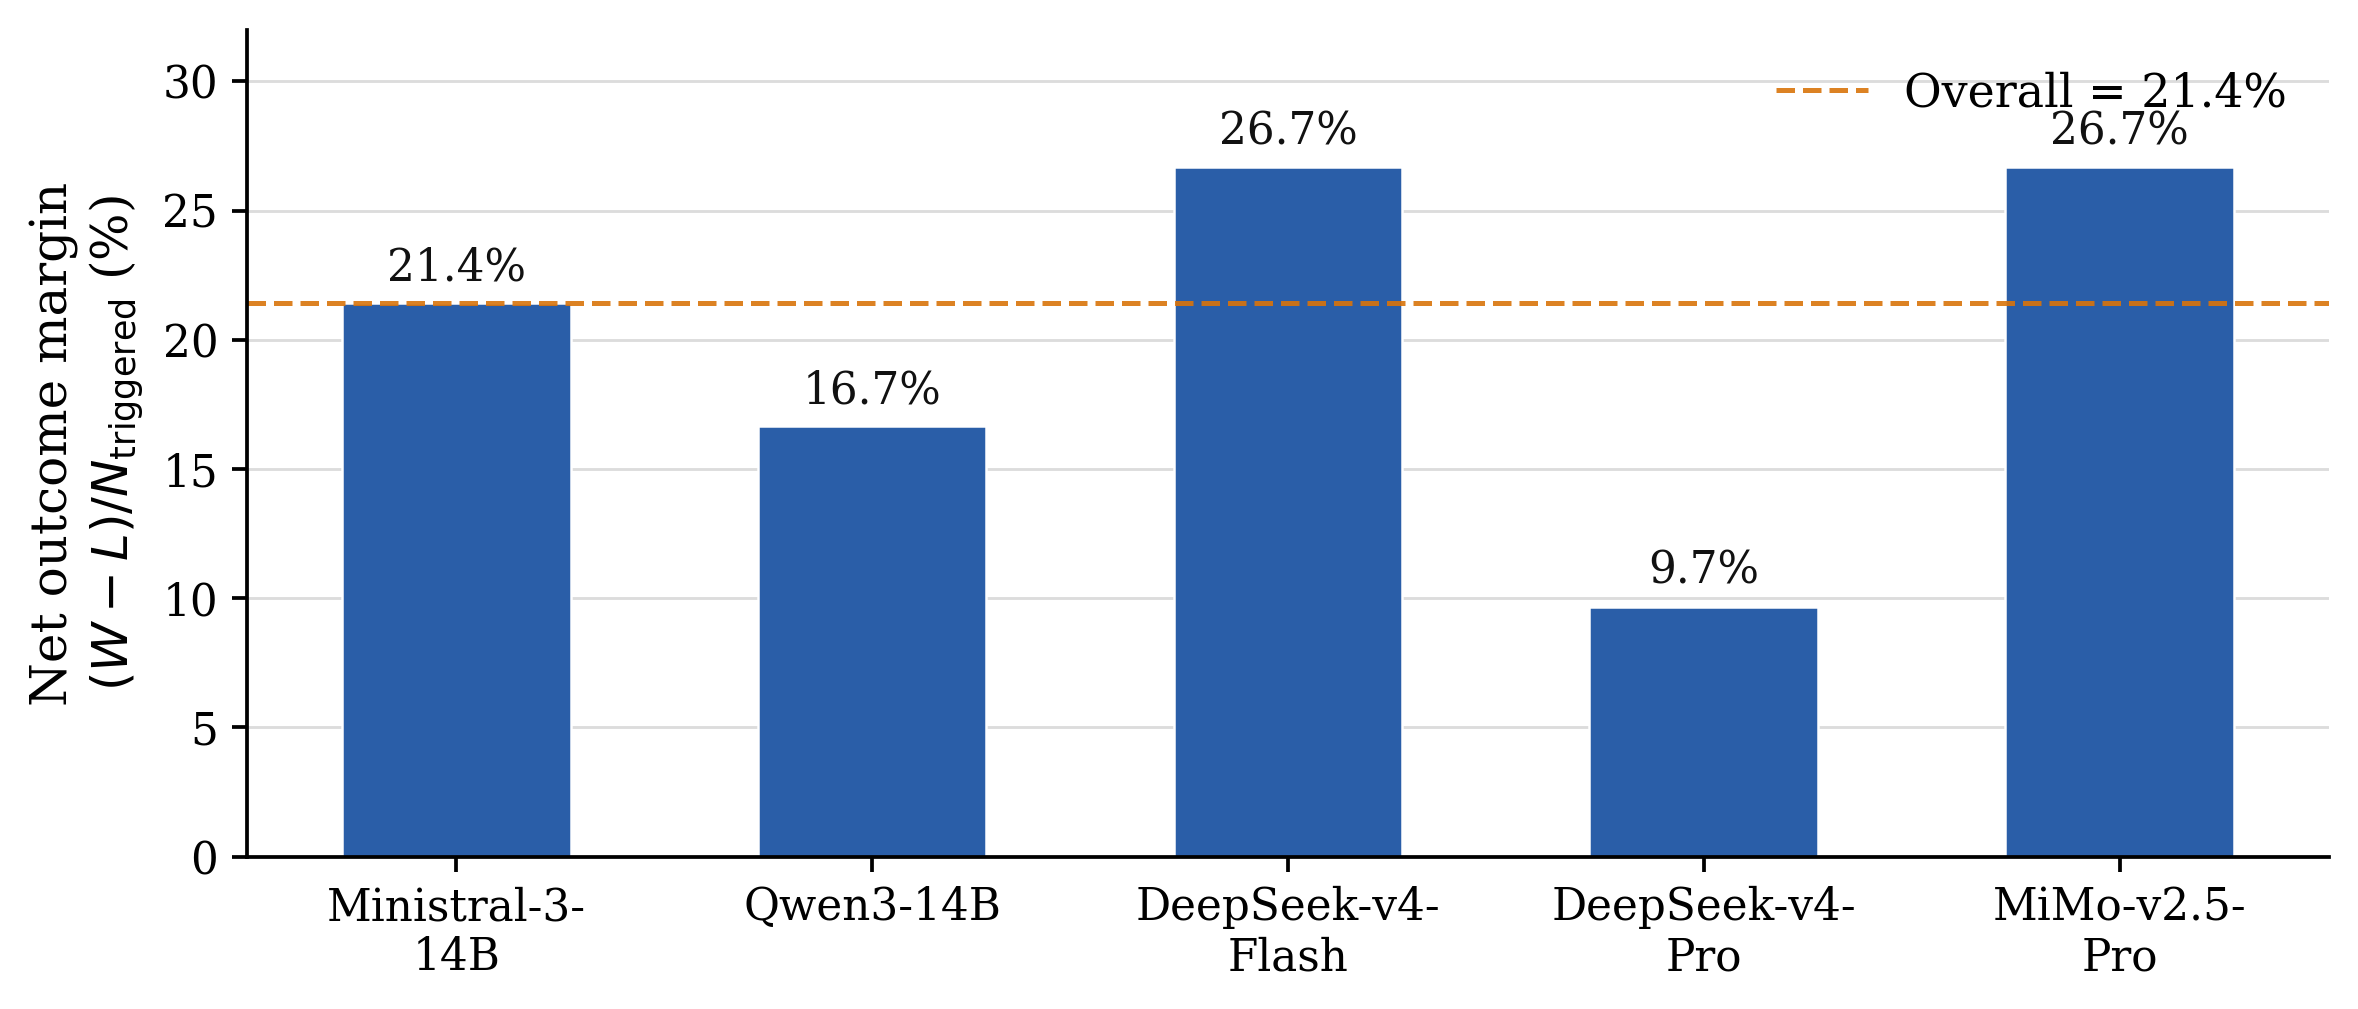
\includegraphics[width=\columnwidth]{figures/fig_statebench_triggered_failure_recovery.png}
\caption{Net outcome margin among triggered STATE-Bench trajectories is positive for every base model, and beneficial interventions outnumber harmful ones on the triggered subset by $(39-9)/140=21.4\%$ overall.}
\label{fig:triggered-failure-recovery}
\end{figure}

\subsection*{Recovery Behavior on Functional Loop-Exposed Trajectories}

To test whether the gain comes from repairing functional loops themselves, we isolate task-runs whose baseline trajectory already contains a functional loop before intervention. Figures~\ref{fig:functional-loop-subset-scores} and \ref{fig:functional-loop-subset-calls} show that scores rise for all five base models while tool calls fall in every case, with the largest score gains on MiMo-v2.5-Pro and DeepSeek-v4-Pro. This validates that LoopBreaker precisely targets the failure mode it is designed for, and raising scores while cutting tool calls rules out gains from simply spending more interaction budget. Overall, these subset results highlight LoopBreaker's deployment behavior on Functional Loop-exposed trajectories, while the same-state experiment in Table~\ref{tab:card-structure-ablation} provides the corresponding controlled evidence for the recovery program itself.

\begin{figure}[!t]
\centering
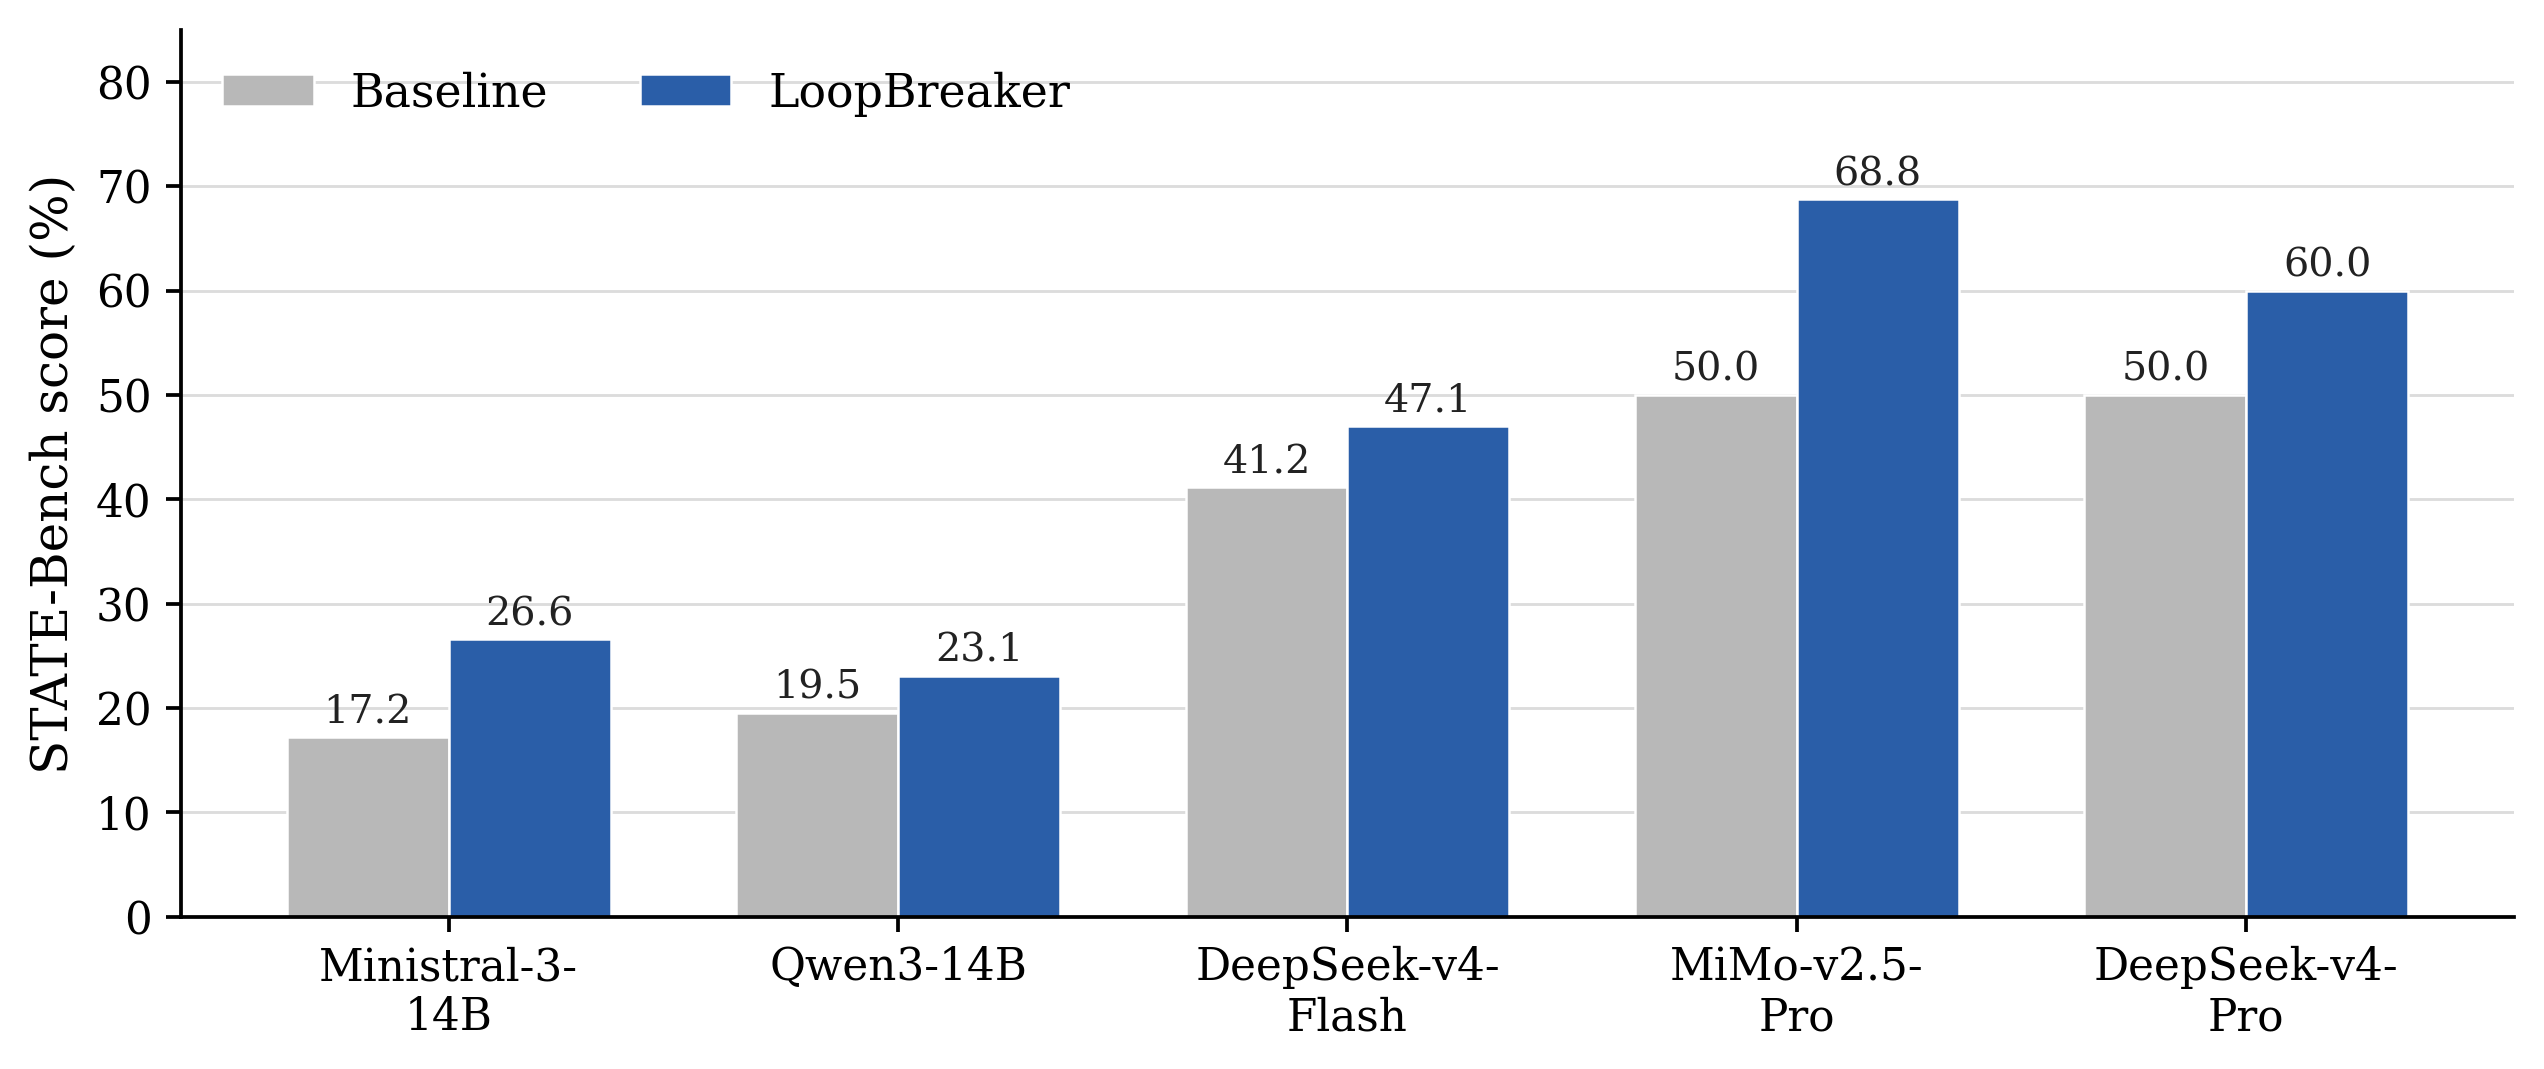
\includegraphics[width=\columnwidth]{figures/fig_statebench_fl_subset_scores.png}
\caption{On task-runs whose baseline trajectory contains a functional loop before intervention, LoopBreaker raises the STATE-Bench score for every base model.}
\label{fig:functional-loop-subset-scores}
\end{figure}

\begin{figure}[!t]
\centering
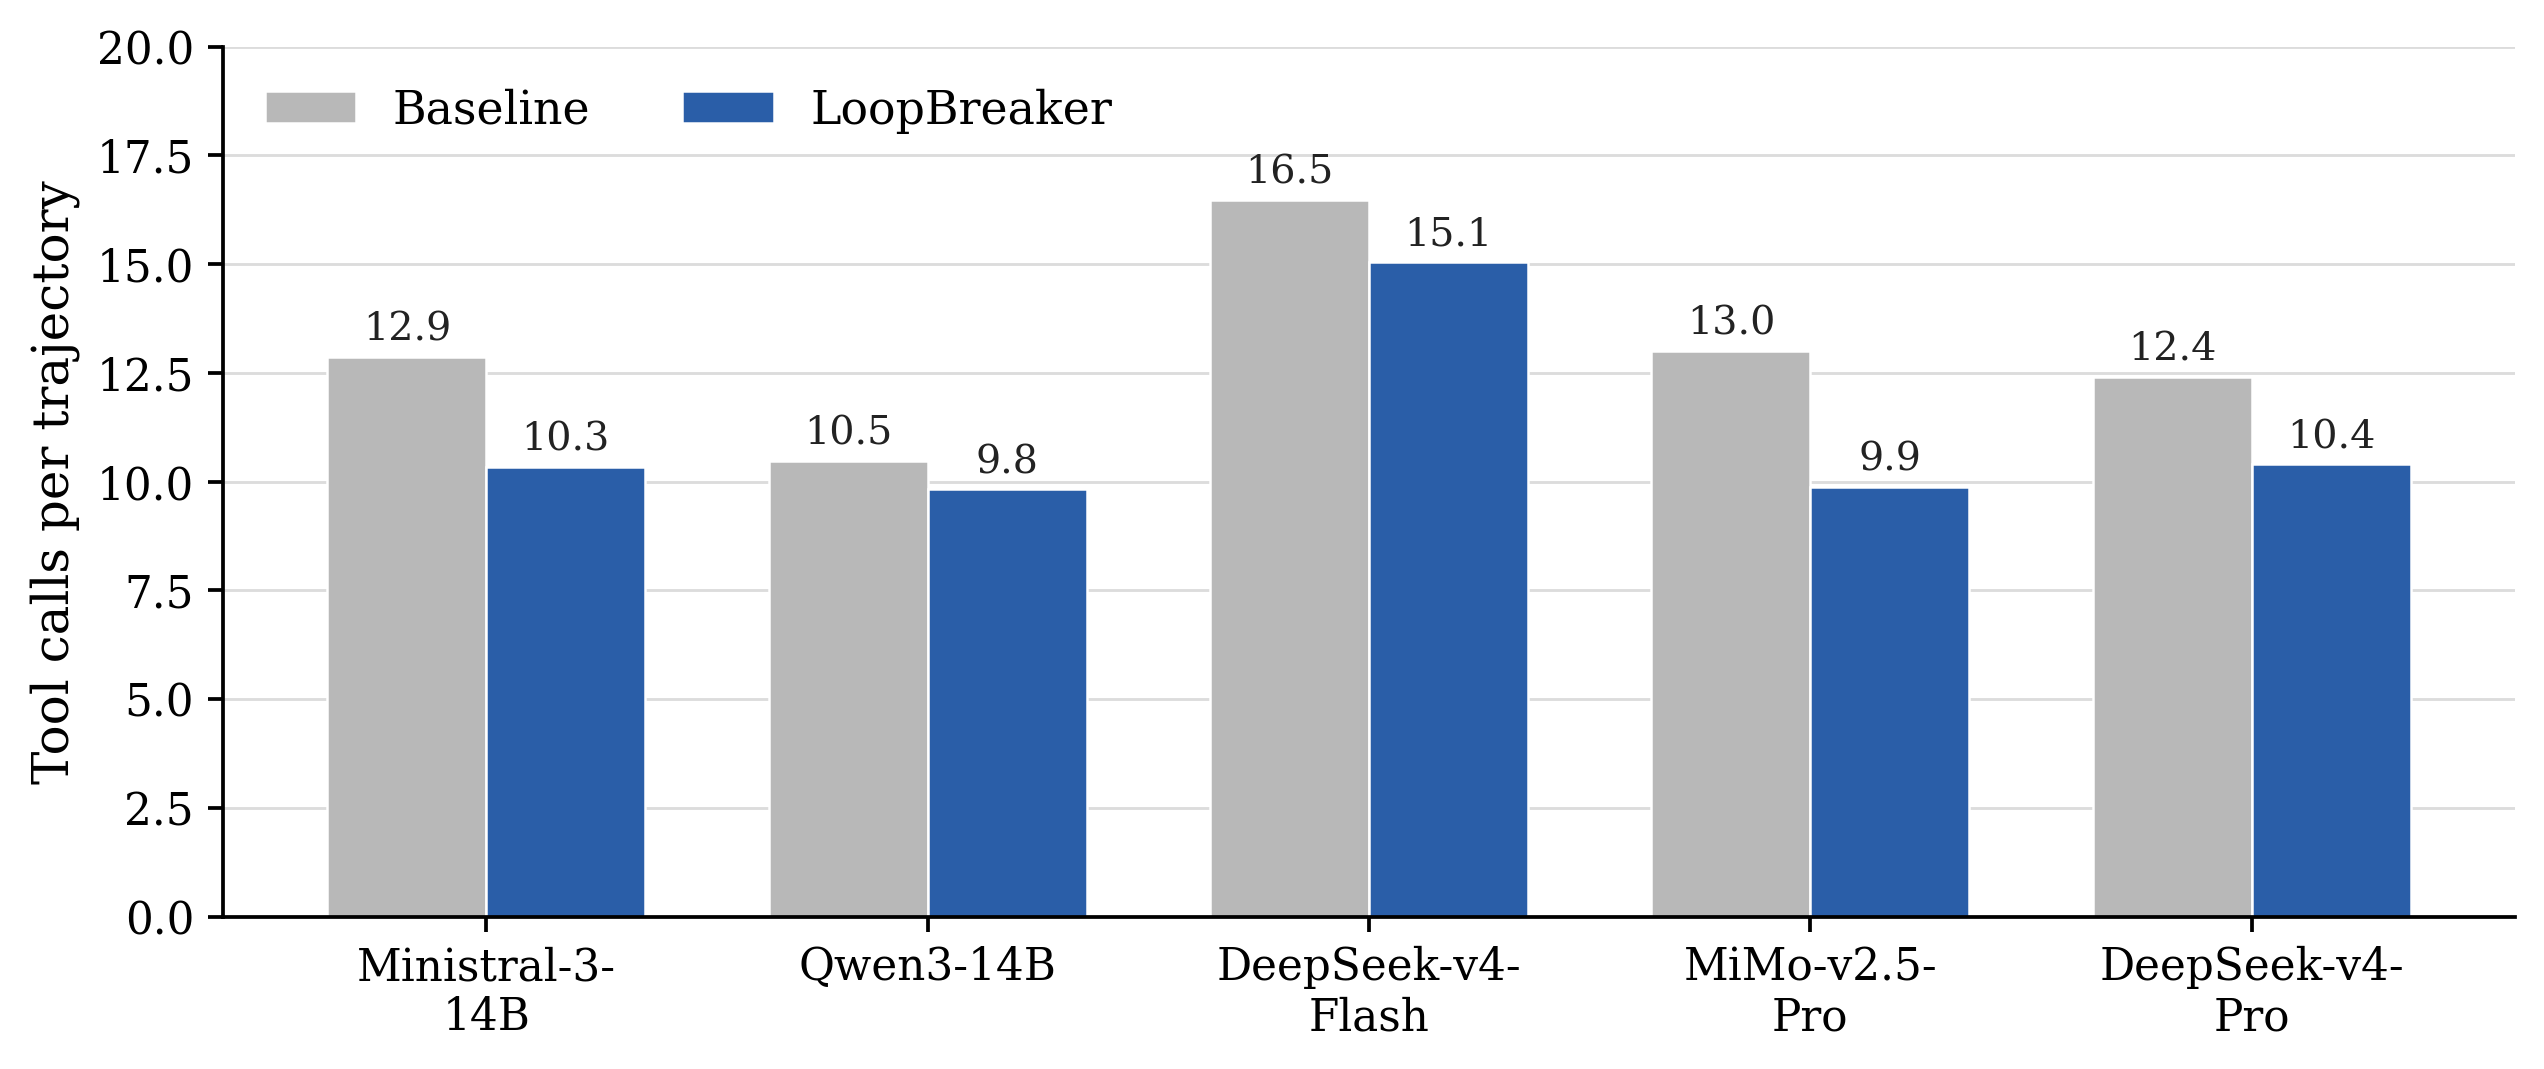
\includegraphics[width=\columnwidth]{figures/fig_statebench_fl_subset_calls.png}
\caption{On the same Functional Loop-exposed task-runs, LoopBreaker reduces the average number of tool calls per trajectory for every base model.}
\label{fig:functional-loop-subset-calls}
\end{figure}


\section{Related Work}

Recent work approaches tool-use failures from several angles. Early-exit methods reduce ineffective behavior by deciding when to halt a stalled trajectory~\citep{lu2025runaway}, while termination alone does not repair a state that a small correction could still resolve. Reflection frameworks such as Reflexion~\citep{shinn2023reflexion} and Self-Refine~\citep{madaan2023selfrefine} accumulate verbal feedback across trials, and CRITIC~\citep{gou2024critic} augments this self-verification with external tools. Test-time replanning generates a fresh recovery plan through another generation step, as in Reasoning Inception~\citep{kim2026rein}, Reinforced Agent~\citep{ta2026reinforced}, and LATS~\citep{zhou2024lats}, while the correction is only as reliable as the underlying model. Workflow and skill memory approaches~\citep{wang2025workflow,wang2025skills} reuse successful trajectories as general-purpose skills, and policy optimization methods learn recovery from execution errors through reinforcement learning~\citep{zhang2026fission,kang2026trace,zhang2026pivot}. Overall, these methods either halt too early, invoke another generation, or require gradient access, and none of them treats the Functional Loop as a distinct recoverable execution state addressed by a validated local program.

In this work, we focus on inference-time recovery from a well-defined execution failure, with the goal of escaping a Functional Loop through a grounded local correction while leaving the base LLM's policy unchanged. Unlike previous approaches that either halt a stalled trajectory, generate an ungrounded replan, or update the model via reinforcement learning, LoopBreaker adopts a more deliberate design by pairing an offline experience compiler with an online selective controller that admits at most one executable Card once a Functional Loop is detected.


\section{Conclusion}

In this paper, we introduced the Functional Loop as a distinct failure mode in tool-using LLMs, in which feedback-visible actions make no task progress and repeat the same unresolved effect. Our analysis across STATE-Bench, DeepPlanning Shopping, and $\tau$-Knowledge shows that Functional Loops are prevalent, are associated with lower task performance, and are not well captured by string-level tool repetition. Along with this observation, we proposed LoopBreaker, a local recovery layer that reuses concrete training-time failures at inference time and admits at most one grounded Recovery Card once a Functional Loop is detected. Across three tool-use benchmarks and nine LLMs, LoopBreaker consistently improves the primary task outcome, and controlled ablations locate the gain in validated Cards under selective admission. LoopBreaker offers a step toward reusing concrete failure experience during tool execution, and complements existing efforts on tool selection, replanning, and policy optimization.

\bibliography{references}

\end{document}
